% Bsp. eines Hauptteils

\chapter{Infrared Sensor}
To achieve our main goal, the autonomous landing, we tried several different sensor. In this Chapter we introduce them, including the problems we were faced and the configurations we did.
\label{sec:infra}


We tried to establish a distance measurement with GP2Y0A60SZLF Infrared Sensor on a Pololu Carrier Board. The Measuring distance of that sensor is 10 to 150 cm. For detailed technical values, please see the sensor chapter or the datasheet.

\section{First steps}
\label{sec:infra1}

Our first action was to check, weather the sensor is working or not. So we need to active the I�C Bus on the Raspberry Pi and set up the Analog Distance Converter (ADS1011), because the Infrared Sensor provides us only a analog output.\\
We did a fast test of the sensor using python, just for checking the sensor is not broken.\\

To gather a bunch of data, we developed I�C and ADC Driver ourselves in C.

\begin{figure}[H]
	\centering\includegraphics[width=0.8\textwidth]{fig/ch-distance_measurement/adc_ir_wiring}
	\caption{Wiring ADC and IR}
	\label{fig:adcirwiring}
\end{figure}



\subsection{ADC Configuration}
\label{sec:adc_conf}

First Hex depends on Starting Conversion + the Input, which Pin to read A0-3,\\
Second Value is PGA (001)=+-4,099V and continuous Mode (0).


These three bytes are written to the ADS1015 to set the config register and start the conversion. 

  l\_writeBuf\_rg24[0] = 1;		\\
	This sets the pointer register to write two bytes to the config register
	
  l\_writeBuf\_rg24[1] = l\_mux\_ui8;   \\
	This sets the 8 MSBs of the config register (bits 15-8) to 11000011
	
  l\_writeBuf\_rg24[2] = 0x23;  		\\
	This sets the 8 LSBs of the config register (bits  7-0) to 00100011\\
	

  %First Hex is sample Rate. (001) sets to 250SPS + Comp Mode (0)\\
  %Second Hex is Comp. config. (0011) disable the comparator\\


The following table shows the Hex values in the direction from top to bottom what is needed for reading a conversion value on the specific inputs. At the empty field, there is no change compared to Input A0.

\begin{table}[H]
\begin{tabular}{|c|c|c|c|c|c|}\hline
												& Input A0 & Input A1 & Input A2 & Input A3\\ \hline
   Slave adress+RW  & 0x49 &  &  & \\ \hline
   PTR register & 0x01 &  & & \\ \hline
   %MSB Config & 0x44 & 0x54 & 0x64 & 0x74  \\ \hline
	MSB Config & 0xC2 & 0xD2 & 0xE2 & 0xF2  \\ \hline
   LSB Config  & 0x23 & & &   \\ \hline
	Slave adress+RW & 0x49 &  &  & \\ \hline
	PTR register & 0x00 &  &  & \\ \hline
	%Slave adress+RW & 0x93 & && \\ \hline
	Data from Slave & 0xXX & 0xXX & 0xXX & 0xXX\\ \hline
	Data from Slave & 0xXX & 0xXX & 0xXX & 0xXX\\ \hline
 \end{tabular}
 \caption{ADC Conversion Read}
 \label{tab:table1}
 \end{table}

MSB:\\
The first hexadecimal value is to start the conversion and depends on the Input, which Pin to read A0-3.\\
The second hexadecimal value is PGA (001)= +-4,099V and continuous Mode (0).\\

LSB:\\
The first hexadecimal value is the sample Rate. (001) sets it to 250SPS + Comp Mode (0).\\
The second hexadecimal value is the Comp. config. (0011) disables the comparator.\\


\section{Measured Values}
\label{sec:Infra2}

With our own logic getting the data from the sensor, we could store as much data we want. Now we were able to get a impression on the jitter and could thing about a good algorithm to get reliable values.

%\begin{floatingfigure}[v]{5cm}
\begin{figure}[H]
	\centering
		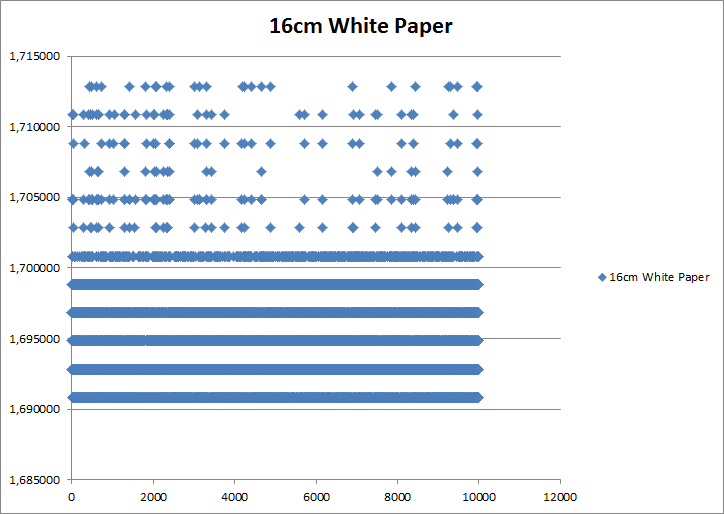
\includegraphics[width=0.8\textwidth]{fig/ch-distance_measurement/WhitePaper16.png}
	\label{fig:WhitePaper16}
	\caption{IR: 16 cm to white paper}
\end{figure}

Gathering 10 000 values while measuring the distance of 16cm on a white paper. We used the white paper to compare the values with them in the datasheet.\\\\

As we changed the distance and the surface, we discover a astonishing fact.\\

\begin{figure}[H]
	\centering
		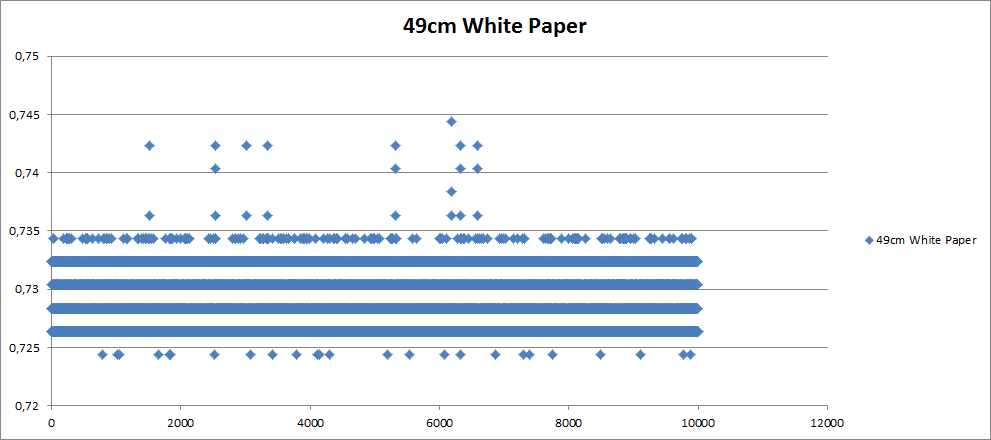
\includegraphics[width=0.8\textwidth]{fig/ch-distance_measurement/WhitePaper49.png}
	\label{fig:WP49}
	\caption{IR: 49 cm to white paper}
\end{figure}

Same measurement on the surface of the table:\\

\begin{figure}[H]
	\centering
		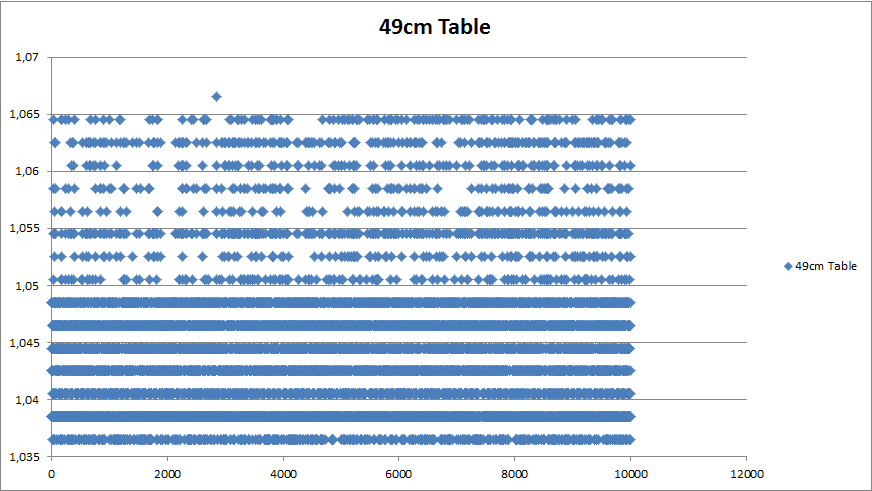
\includegraphics[width=0.8\textwidth]{fig/ch-distance_measurement/Table49.png}
		\caption{IR: 49 cm to table}
	\label{fig:Table49}
\end{figure}

As you see, the measurements on different surfaces are highly varying. At 49cm we got the following rough values:\\

White Paper: ~0,73 V\\
Desk Surface: ~1,42 V

\begin{figure}[H]
	\centering
		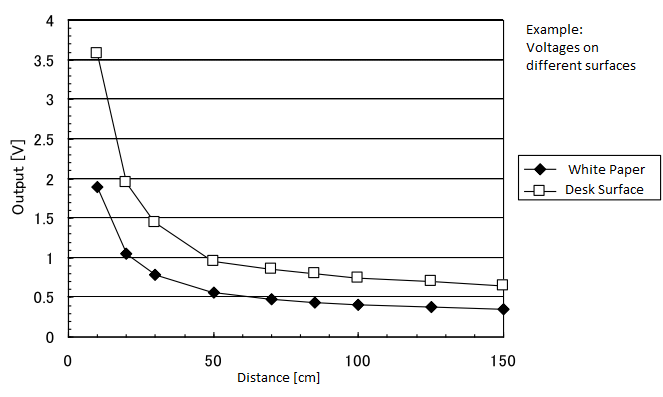
\includegraphics[width=0.8\textwidth]{fig/ch-distance_measurement/Surfaces_Voltages.png}
	\label{fig:WP49}
	\caption{IR: Sensor values (voltages) on different surfaces}
\end{figure}

\newpage
%\underline{2 surfaces and 2 distances}
2 Surfaces and 2 Distances:
\begin{figure}[H]
	\centering
		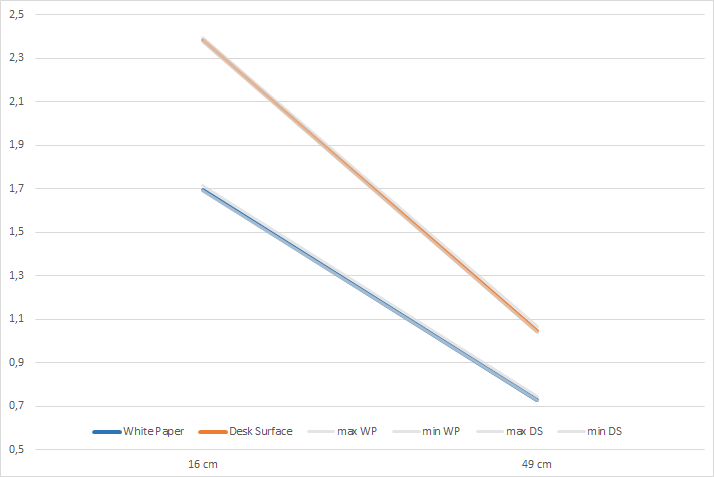
\includegraphics[width=1.0\textwidth]{fig/ch-distance_measurement/Surfaces_Compared.png}
	\label{fig:IR_Surf}
	\caption{IR: Compared Voltages on two surfaces}
\end{figure}

We only measured 2 different distances in order to check the functionality of the sensor. The grey lines shows the jitter which we measured. 

\section{Conclusion}
\label{sec:IRCon}

As we could not guarantee a good flying with changing surfaces, we decided to stop chasing a solution with the IR Sensor.


\chapter{Ultrasonic Distance Sensor}
\label{cha:ultra}

Our next approach was, measuring the distance with a ultrasonic distance sensor. In a meeting we agreed on using 3 ultrasonic sensor to measure the distance to ground, because a single sensor is imprecise. We hoped that a sensor fusion of 3 ultrasonics will bring us better values.\\

While searching for theses sensors, we found a relatively cheap Laser Sensor. After a short consultation, we decided to go with that one. So Ultrasonic was discarded, before start.



\chapter{LIDAR Laser Sensor}
\label{cha:laser}

LIDAR-Lite Laser Distance Sensor\\
Model LL-905-PIN-01\\

Performance\\
Range: 0-20m LED Emitter\\
Range: 0-60m Laser Emitter\\

Interfaces\\
- I$^2$C\\
- PWM\\

For detailed technical values, please see the sensor chapter or the datasheet.\\

\section{Connecting the sensor with I$^2$C}
\label{sec:lascon}

Because there is no proper input for a PWM signal, we used the I$^2$C Bus to connect the laser sensor. As the sensor does not support fast I$^2$C mode, which we need, we decided to use the second I$^2$C on the Raspberry Pi. This bus is orginally located on the camera port with an FPC (flexible printed circuit) Connector. We managed it to redirect it to the normal Pins on the board. See Chapter xxxxxx.

\begin{figure}[H]
	\centering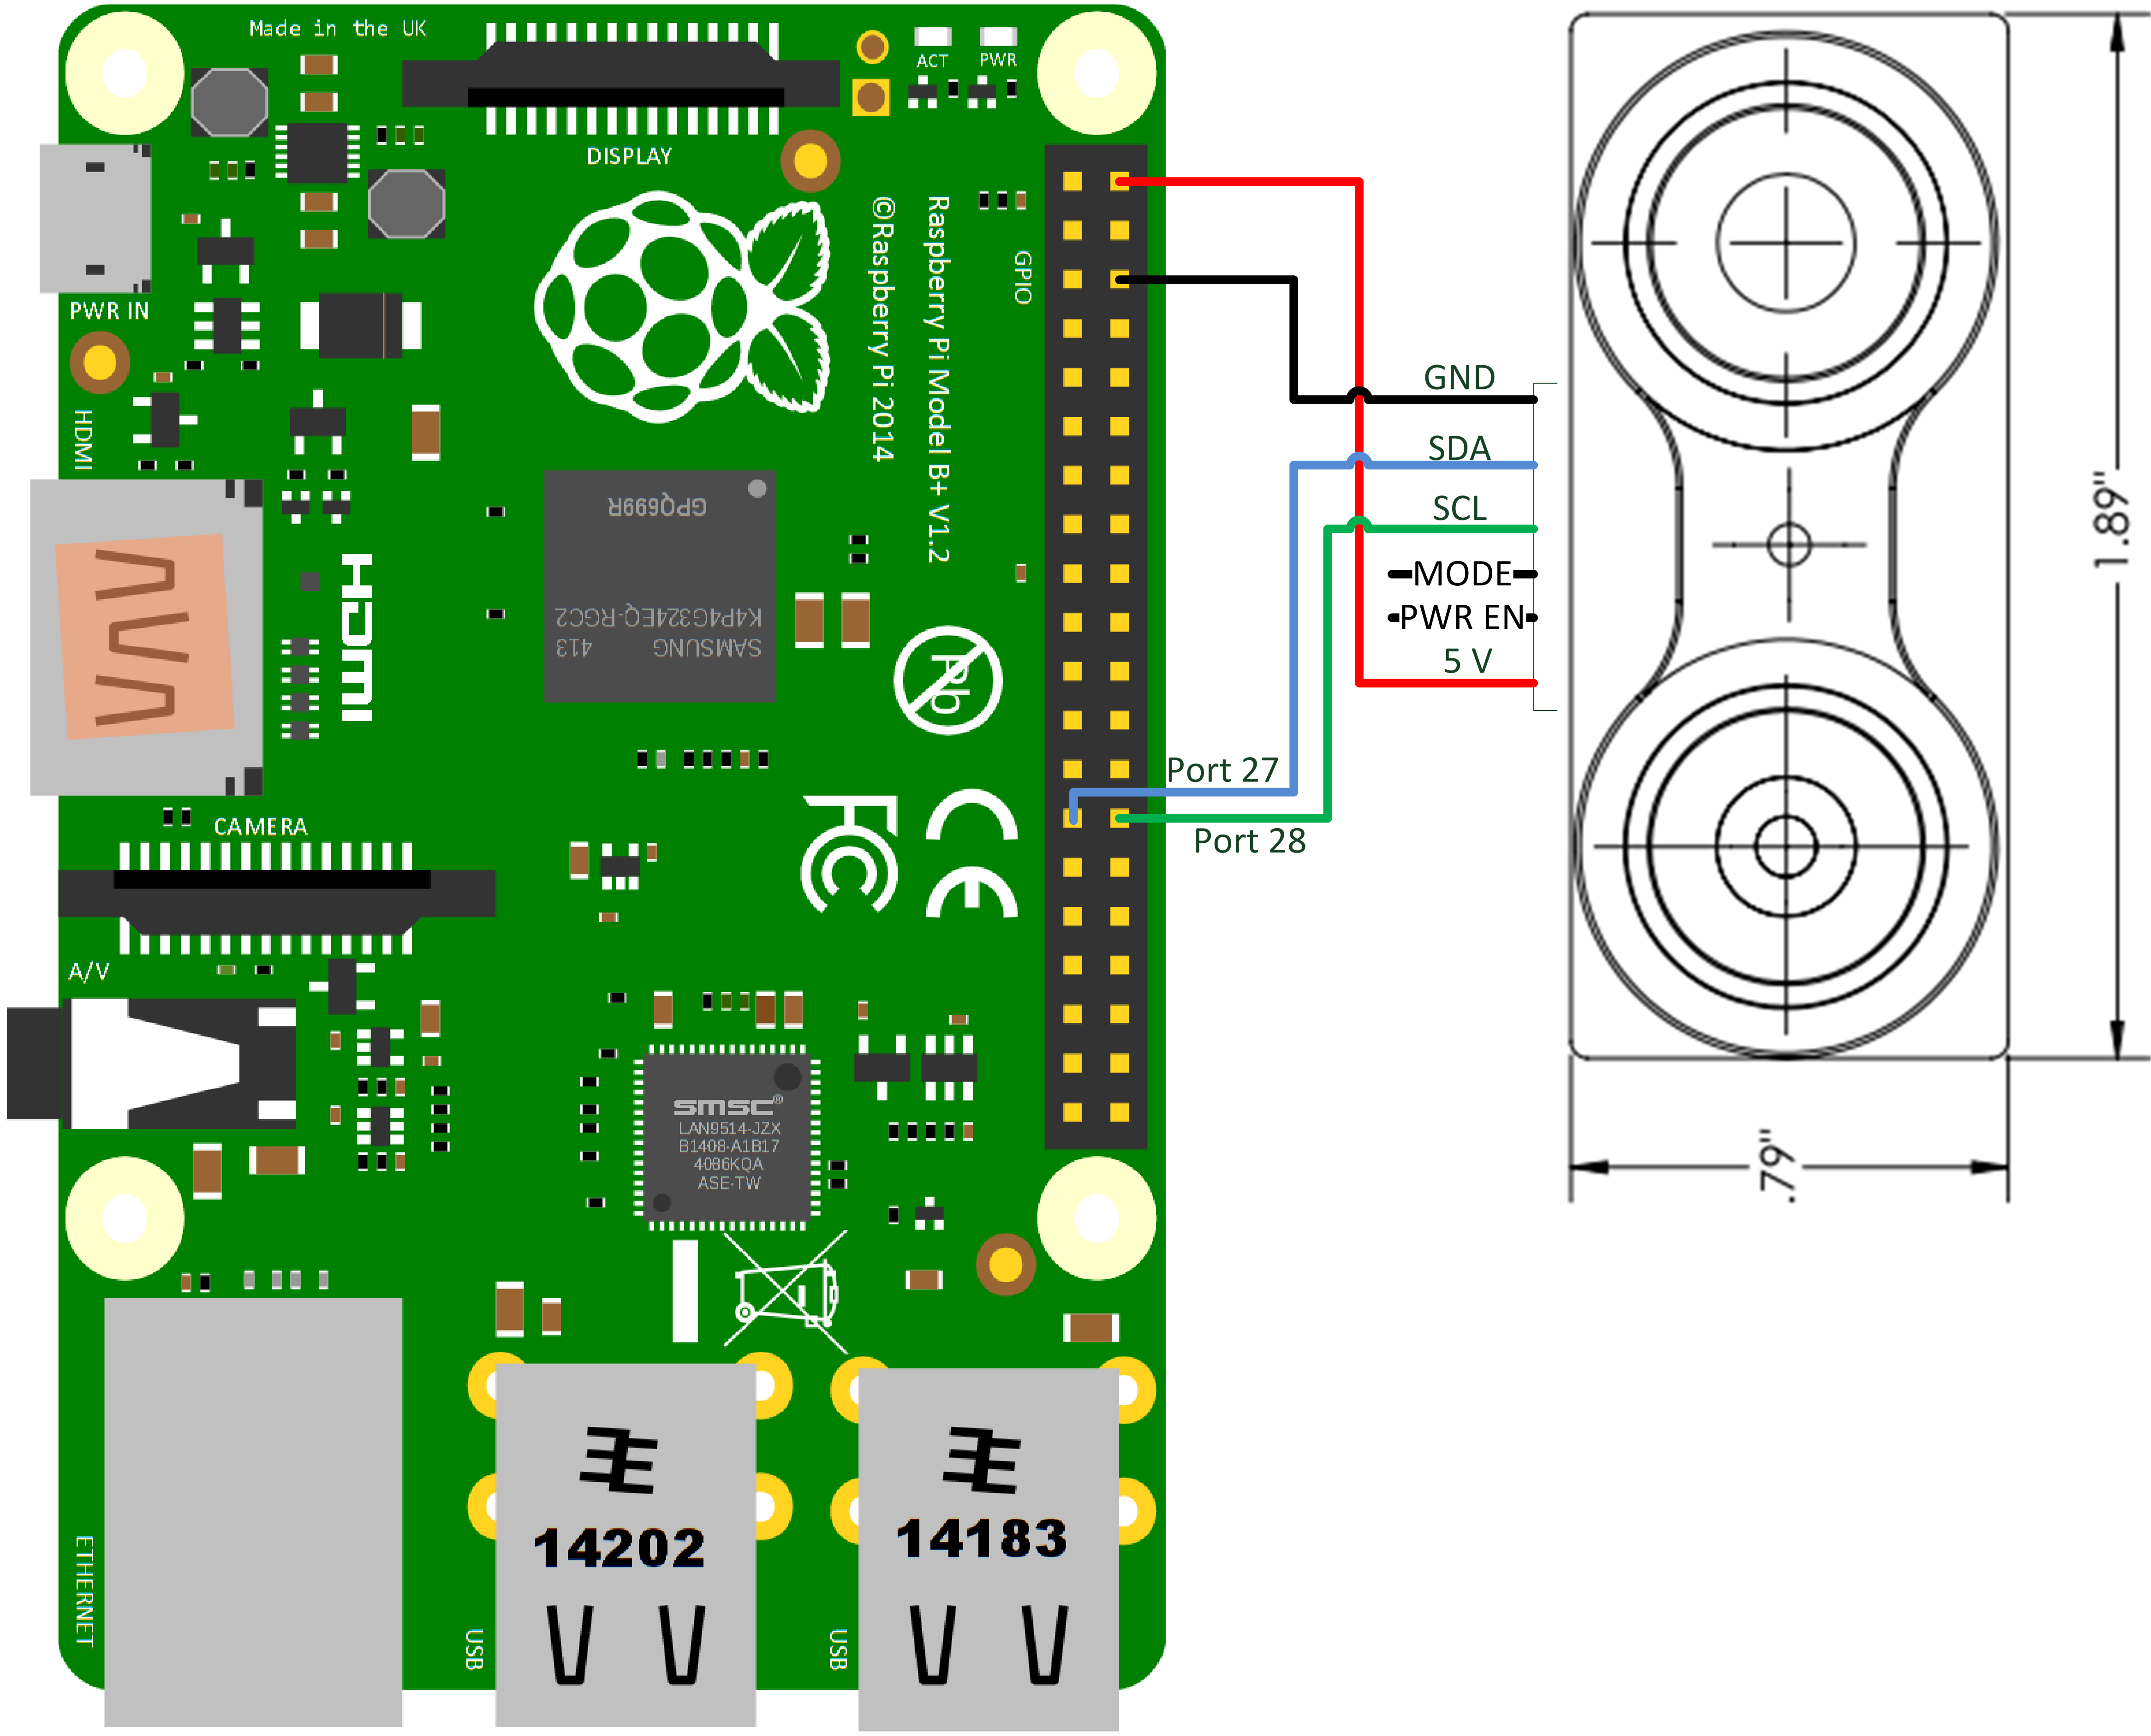
\includegraphics[width=0.8\textwidth]{fig/ch-distance_measurement/lidar_wiring}
	\caption{Wiring LIDAR}
	\label{fig:lidarwiring}
\end{figure}

\section{First steps}
\label{sec:lasfirst}

Quick Start Guide 

1.  Make Power and I2C Data Connections as per J1 connector pin out diagram.  Pins 2 \& 3 are optional connections and not required. \\
2.  Initialization:  Apply Power to the Module. The sensor operates at 4.75-5.5V DC Nominal, Maximum 6V DC.\\
3.  Measurement: Write register 0x00 with value 0x04 (This performs a DC stabilization cycle, Signal Acquisition, Data processing). Refer to the section "`I2C Protocol Summary"' in this manual for more information about I2C Communications.\\
4.  Periodically poll the unit and wait until an ACK is received. The unit responds to read or write requests with a NACK when the sensor is busy processing a command or performing a measurement. 
(Optionally, wait approx. 20 milliseconds after acquisition and then proceed to read of high and low bytes) \\
5.  Read:  register 0x0f, returns the upper 8 bits of distance in cm, register 0x10, returns the lower 8 bits of 
distance in cm.  (Optionally a 2-Byte read starting at 0x8f can be done) 


\section{Measured Values}
\label{sec:lasvalues}

To test and verify functionality and accuracy of the sensor a series of tests was done. The following figure shows the deviation of the sensor of different surfaces. Each bar represents the mean value of at least ten measurements. As you can see at a distance of app. 150 cm the deviation is only 2 cm. With this tests the given accuracy of +/- 2.5 cm (see datasheet) gets confirmed.

\begin{figure}[H]
	\centering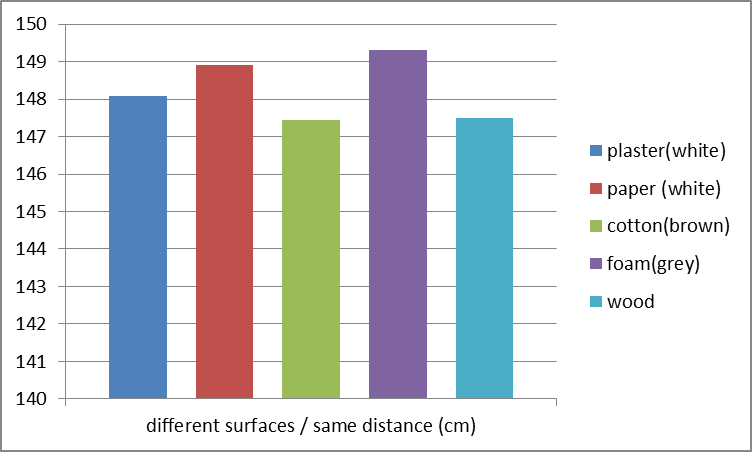
\includegraphics[width=0.75\textwidth]{fig/ch-distance_measurement/laser_mess}
	\caption{Laser measured values}
	\label{fig:lasermess}
\end{figure}
\newpage
To verify a correct distance measurement while flying also different angles to ground were tested. In a set of tests with an angle between 90\textdegree (vertically) and 10\textdegree  and a distance range of app. 200cm the sensor returned valid and correct values.

\begin{figure}[H]
	\centering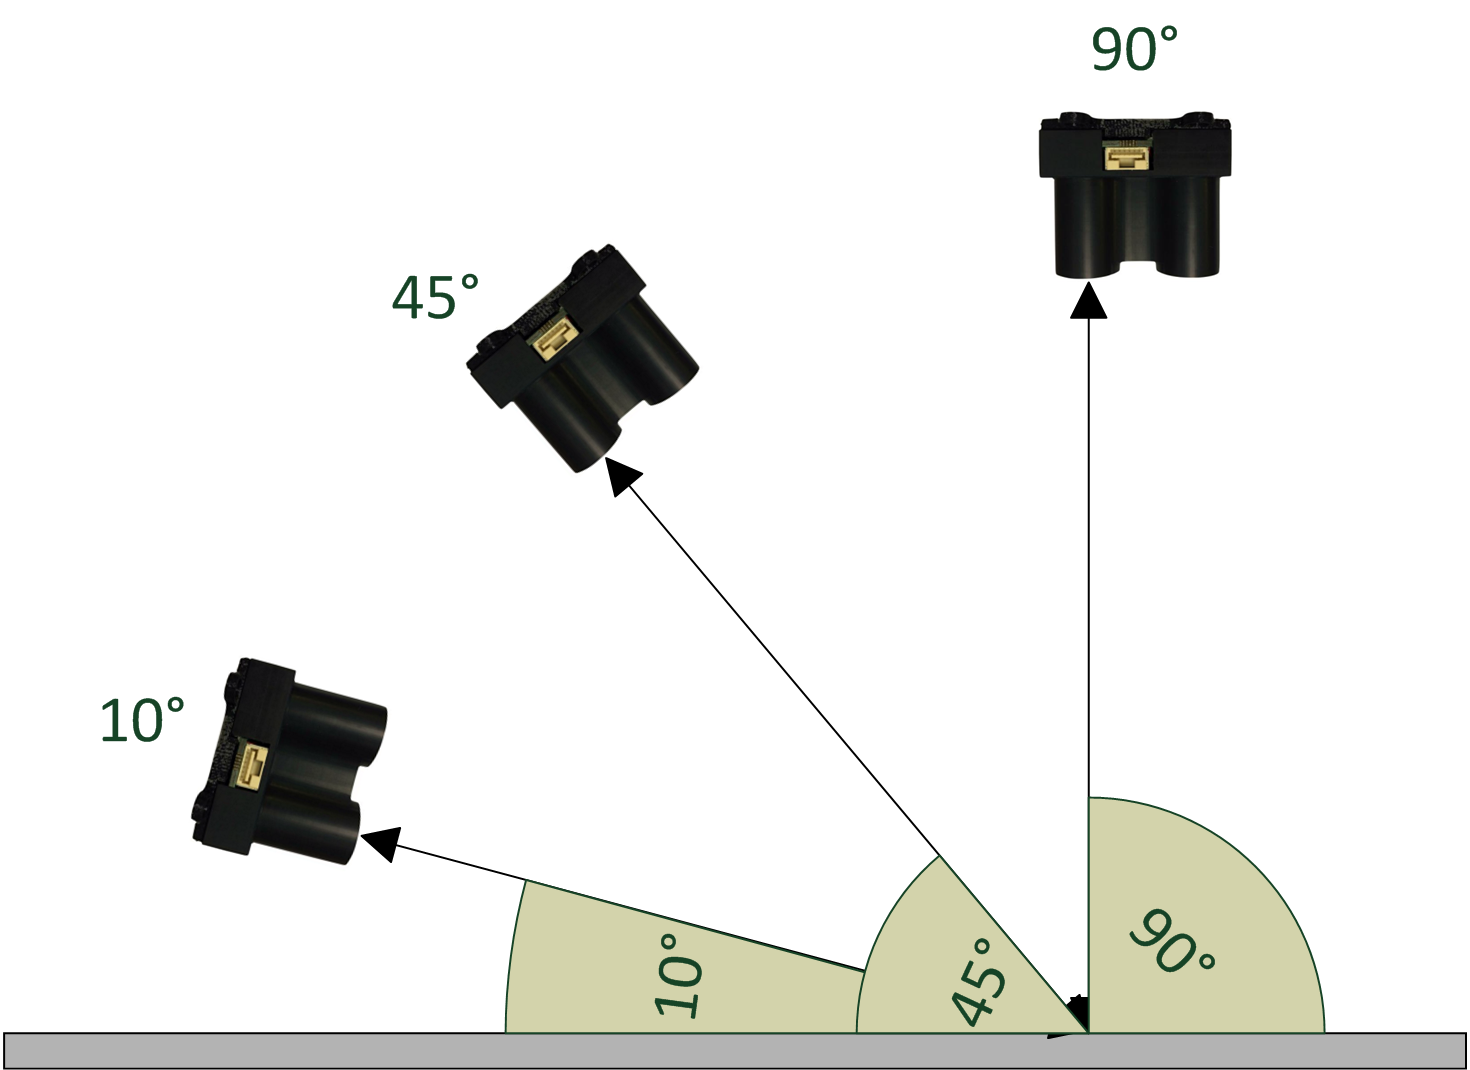
\includegraphics[width=0.5\textwidth]{fig/ch-distance_measurement/angles}
	\caption{different measured angles}
	\label{fig:angle}
\end{figure}

\section{conclusion}
\label{sec:lasconlu}

The Laser sensor provides us reliable distance values, independent from the surface or material we measure at. The measurement get's a little bit worse below 20 cm, but with a estimated build in height of 10 cm at the quadrocopter, we can along with that.

We recommend to pursuit future autonomous landing approaches, with that sensor.

Regarding the Class 1 Laser Specification, there is no danger in using the sensor, even when looking straight in the laser.


